\documentclass[letterpaper]{article}
\usepackage{amssymb}
\usepackage{fullpage}
\usepackage{amsmath}
\usepackage{epsfig,float,alltt}
\usepackage{psfrag,xr}
\usepackage[T1]{fontenc}
\usepackage{url}


\begin{document}

\newcommand{\trace}{\mathrm{trace}}
\newcommand{\real}{\mathbb R}  % real numbers  {I\!\!R}
\newcommand{\nat}{\mathbb R}   % Natural numbers {I\!\!N}
\newcommand{\cp}{\mathbb C}    % complex numbers  {I\!\!\!\!C}
\newcommand{\ds}{\displaystyle}
\newcommand{\mf}[2]{\frac{\ds #1}{\ds #2}}
\newcommand{\book}[2]{{Luenberger, Page~#1, }{Prob.~#2}}
\newcommand{\spanof}[1]{\textrm{span} \{ #1 \}}
\parindent 0pt


\begin{center}
{\large \bf HW \# 04 Solutions}
\end{center}

\vspace*{1cm}


%Prob. 1 Representation and change of basis matrix
\noindent \textbf{Problem 1:}
\begin{enumerate}
\setlength{\itemsep}{.1in}
\renewcommand{\labelenumi}{(\alph{enumi})}
\item By inspection,
$$\boldsymbol{r}(x)=2\boldsymbol{p}_0 + 3\boldsymbol{p}_1 - \boldsymbol{p}_2$$
and thus
$$\big[\boldsymbol{r}(x)\big]_{\cal S} = \begin{bmatrix} 2 \\ 3 \\ -1 \end{bmatrix}$$

\item We seek coefficients $\alpha_0 , \alpha_1 , \alpha_2$ such that
$$\boldsymbol{r}(x)=\alpha_0 \boldsymbol{q}_0 + \alpha_1 \boldsymbol{q}_1 + \alpha_2 \boldsymbol{q}_2$$
hence
$$\begin{aligned}
    2+3x-x^2 &= \alpha_0 + \alpha_1 (1-x) + \alpha_2 (x+x^2) \\
             &= ( \alpha_0 + \alpha_1 ) + ( \alpha_2 - \alpha_1 ) x + \alpha_2 x^2
\end{aligned}$$
Therefore
$$\begin{aligned}
    \alpha_0 + \alpha_1 &= 2 \\
    \alpha_2 - \alpha_1 &= 3 \\
    \alpha_2 &= -1
\end{aligned}$$
which yields
$$\begin{aligned}
    \alpha_0 &= 6 \\
    \alpha_1 &= -4 \\
    \alpha_2 &= -1
\end{aligned}$$
In other words,
$$\big[\boldsymbol{r}(x)\big]_{\cal Q} = \begin{bmatrix} 6 \\ -4 \\ -1 \end{bmatrix}$$

\item We define $\bar{P}=P^{-1}$, and compute $\bar{P}=[\bar{P}_1,\bar{P}_2,\bar{P}_3]$, where
$$\begin{aligned}
    \bar{P}_1 &= \big[\boldsymbol{q}_0\big]_{\cal S} = \begin{bmatrix} 1 \\ 0 \\ 0 \end{bmatrix} \\
    \bar{P}_2 &= \big[\boldsymbol{q}_1\big]_{\cal S} = \begin{bmatrix} 1 \\ -1 \\ 0 \end{bmatrix} \\
    \bar{P}_3 &= \big[\boldsymbol{q}_2\big]_{\cal S} = \begin{bmatrix} 0 \\ 1 \\ 1 \end{bmatrix} \\
\end{aligned}$$
Hence,
$$P=\begin{bmatrix} 1 & 1 & 0 \\ 0 & -1 & 1 \\ 0 & 0 & 1\end{bmatrix}^{-1} =  \begin{bmatrix} 1 & 1 & -1 \\ 0 & -1 & 1 \\ 0 & 0 & 1\end{bmatrix}$$
\end{enumerate}

\bigskip

%Prob. 2 e-values and e-vectors
\noindent \textbf{Problem 2:}
By inspection, the e-values are $\lambda_1 = 1, \lambda_2 = 2, \lambda_3 = 3$.
$$\begin{aligned}
(A_3 - \lambda_1 I)&=\left[ \begin{array}{ccc} 0 & 4 & 10 \\ 0 & 1 & 0 \\ 0& 0& 2 \end{array} \right] \\
0 &= (A_3 - \lambda_1 I) v^1 \Rightarrow v^1 = \begin{bmatrix} 1 \\ 0 \\ 0 \end{bmatrix} \\
(A_3 - \lambda_2 I)&=\left[ \begin{array}{ccc} -1 & 4 & 10 \\ 0 & 0 & 0 \\ 0& 0& 1 \end{array} \right] \\
0 &= (A_3 - \lambda_2 I) v^2 \Rightarrow v^2 = \begin{bmatrix} 4 \\ 1 \\ 0 \end{bmatrix} \\
(A_3 - \lambda_3 I)&=\left[ \begin{array}{ccc} -2 & 4 & 10 \\ 0 & -1 & 0 \\ 0& 0& 0 \end{array} \right] \\
0 &= (A_3 - \lambda_3 I) v^3 \Rightarrow v^3 = \begin{bmatrix} 5 \\ 0 \\ 1 \end{bmatrix}
\end{aligned}$$
The e-vectors are NOT unique. Any non-zero multiples are also e-vectors. \medskip \\
Because the e-values are distinct, the e-vectors should be linearly independent.
$$\begin{aligned}
0&=\alpha_1 v^1 + \alpha_2 v^2 + \alpha_3 v^3 = \left[\begin{array}{c|c|c} v^1 & v^2 & v^3\end{array}\right] \begin{bmatrix} \alpha_1 \\ \alpha_2 \\ \alpha_3 \end{bmatrix} \\
V &= \left[\begin{array}{c|c|c} v^1 & v^2 & v^3\end{array}\right] = \left[\begin{array}{ccc} 1 & 4 & 5\\ 0 & 1 & 0 \\ 0& 0& 1 \end{array}\right]
\end{aligned}$$
and $\det(V) = 1 \not= 0$. Hence, only solution is $\alpha_1 = \alpha_2 = \alpha_3 =0$, and indeed, the set $\{v^1 , v^2 , v^3 \}$ is linearly independent.

\input{../Prob2.txt}

\bigskip

\noindent \textbf{Problem 3:}
By inspection, $\lambda_1 = 3, \lambda_2 = 3, \lambda_3 = 2$ and we have repeated e-values.
$$\begin{aligned}
(A_4 - \lambda_1 I)&=\left[ \begin{array}{ccc} 0 & 1 & 0 \\ 0 & 0 & 0 \\ 0& 0& -1 \end{array} \right] \\
0 &= (A_4 - \lambda_1 I) v^1 \Rightarrow v^1 = \begin{bmatrix} 1 \\ 0 \\ 0 \end{bmatrix} \end{aligned}$$
Of course, the same is true for $\lambda_2$, and thus $v^2$ is not independent of $v^1$.
\medskip \\
$\therefore$ No basis of e-vectors is possible.

\bigskip

\noindent \textbf{Problem 4:}
We use two facts: \medskip \\
$(i)~~ P^{-1} \cdot P = I $. \medskip \\
$(ii)~ \det(M_1 M_2 ) = \det(M_1)\det(M_2)$  for compatible matrices $M_i$.
$$\begin{aligned}\det(\lambda I-B) &= \det(\lambda I - P^{-1}AP) \\
                                    &= \det(\lambda P^{-1}P - P^{-1}AP) \\
                                    &= \det(P^{-1}[\lambda I - A]P) \\
                                    &= \det(P^{-1})\det(\lambda I - A)\det(P) \\
\end{aligned}$$
But $1=\det(I)=\det(P^{-1}P)=\det(P^{-1})\det(P)$, and thus                                    $$\det(\lambda I - P^{-1} AP) = \det(\lambda I -A)$$

\bigskip

\noindent \textbf{Problem 5:}
We translate $Av^i = \lambda_i v^i$ into the matrix formula
$$AP = P\Lambda$$
where $P=\left[\begin{array}{c|c|c} v^1 & \cdots & v^n\end{array}\right]$ and
$\Lambda =\left[\begin{array}{ccc} \lambda_1 & &\raisebox{-1.7ex}[0pt]{\huge0} \\
                                   & \ddots & \\
                                  \text{\huge0} & & \lambda_n
                                  \end{array}\right]$. \medskip \\
$P$ is invertible if, and only if, its columns are linearly independent, which we know is the case when the e-values are distinct.
$$\therefore P^{-1}AP=\Lambda$$
is the general result, and the specific result for $A_3$ is
$$\left[ \begin{array}{ccc} 1 & 4 & 5 \\ 0 & 1 & 0 \\ 0& 0& 1 \end{array} \right] ^{-1}
    \left[ \begin{array}{ccc} 1 & 4 & 10 \\ 0 & 2 & 0 \\ 0& 0& 3 \end{array} \right]
    \left[ \begin{array}{ccc} 1 & 4 & 5 \\ 0 & 1 & 0 \\ 0& 0& 1 \end{array} \right]=
    \left[ \begin{array}{ccc} 1 & 0 & 0 \\ 0 & 2 & 0 \\ 0& 0& 3 \end{array} \right]$$

\underline{Remark} You did not have to provide the general result!

\bigskip

\noindent \textbf{Problem 6:}

\begin{enumerate}
\setlength{\itemsep}{.1in}
\renewcommand{\labelenumi}{(\alph{enumi})}

\item Checking $L(M_1+M_2) = L(M_1) + L(M_2)$ and $L(\alpha M) = \alpha L(M)$ is immediate and not given.

\item $A=\left[\begin{array}{c|c|c|c} A_1 & A_2 & A_3 & A_4\end{array}\right]$ where
$$A_i=\big[L(u^i)\big]_{\{u\}}$$
$\{u\}=\{E^{11},E^{12},E^{21},E^{22}\}$. \medskip \\
\underline{We compute}

\setlength{\jot}{8pt}
\begin{align*}
L(E^{11})&=\left[\begin{array}{cc} 1 & 0 \\ 0 &0\end{array}\right]=1 \cdot E^{11}+0 \cdot E^{12}+0 \cdot E^{21}+0 \cdot E^{22} \\
L(E^{12})&=\left[\begin{array}{cc} 0 & \frac{1}{2} \\ \frac{1}{2} & 0\end{array}\right]=0 \cdot E^{11}+\frac{1}{2} \cdot E^{12}+\frac{1}{2} \cdot E^{21}+0 \cdot E^{22} \\
L(E^{21})&= L(E^{12}) \\
L(E^{11})&=\left[\begin{array}{cc} 0 & 0 \\ 0 &1\end{array}\right]=0 \cdot E^{11}+0 \cdot E^{12}+0 \cdot E^{21}+1 \cdot E^{22}
\end{align*}
\renewcommand{\arraystretch}{1.25}
$$\therefore A=\left[\begin{array}{cccc} 1&0&0&0 \\0&\frac{1}{2}&\frac{1}{2}&0 \\ 0&\frac{1}{2}&\frac{1}{2}&0 \\ 0&0&0&1\end{array}\right]$$

\end{enumerate}

\newpage

\noindent \textbf{Problem 7:}
\begin{enumerate}
\setlength{\itemsep}{.1in}
\renewcommand{\labelenumi}{(\alph{enumi})}
\item We use the basis
$$\left\{e^1=\begin{bmatrix} 1\\ 0 \\ \vdots \\0 \end{bmatrix},\cdots,e^n = \begin{bmatrix}0\\ \vdots \\ 0 \\1 \end{bmatrix}\right\}$$
$\hat{A}_i=\big[L(e^i)\big]_{\{e\}}$, $\hat{A}=\left[\begin{array}{c|c|c} \hat{A}_1 & \cdots & \hat{A}_n\end{array}\right]$, $L(e^i)=Ae^i=$ the i-th column of $A$. \\
Hence $\boxed{\hat{A}=A}$.

\item Let $\{\lambda_1,\cdots,\lambda_n\}$ be the e-values, which are assumed to be distinct, and let $\{v^1,\cdots,v^n\}$ be the e-vectors, which are consequently linearly independent and form a basis for $({\cp}^n,\cp)$. We define
    $$\hat{A}_i=\big[L(v^i)\big]_{\{v\}}$$
$L(v^i)=Av^i=\lambda_i v^i$,and thus
    $$\hat{A}_i=\lambda_i e^i$$
and therefore
$$\hat{A}=\Lambda =\left[\begin{array}{ccc} \lambda_1 & &\raisebox{-1.7ex}[0pt]{\huge0} \\
                                   & \ddots & \\
                                  \text{\huge0} & & \lambda_n
                                  \end{array}\right]$$
\end{enumerate}

\bigskip

\noindent \textbf{Problem 8:}
\begin{enumerate}
\setlength{\itemsep}{.1in}
\renewcommand{\labelenumi}{(\alph{enumi})}
\item We write $\hat{f}(t_i)=\alpha_0+\alpha_1(t_i)+\cdots+\alpha_5(t_i)^5$ and form the matrices
$$A=\left[\begin{array}{ccccc} 1 & t_1 & (t_1)^2 & \cdots & (t_1)^5 \\
\vdots & \vdots & \vdots & & \vdots \\
1 & t_N & (t_N)^2 & \cdots & (t_N)^5
\end{array}\right], b=\begin{bmatrix}f(t_1) \\ \vdots \\ f(t_N) \end{bmatrix} \text{and } \alpha=\begin{bmatrix}\alpha_0 \\ \vdots \\ \alpha_5 \end{bmatrix}$$
From the handout, we obtain
$$\hat{\alpha} = (A^T A)^{-1} A^T b =\begin{bmatrix}
-0.037 \\ 2.216 \\ 2.89 \\ -11.23 \\ 7.7 \\ -1.54\end{bmatrix}$$

\begin{figure}[h]
\centering
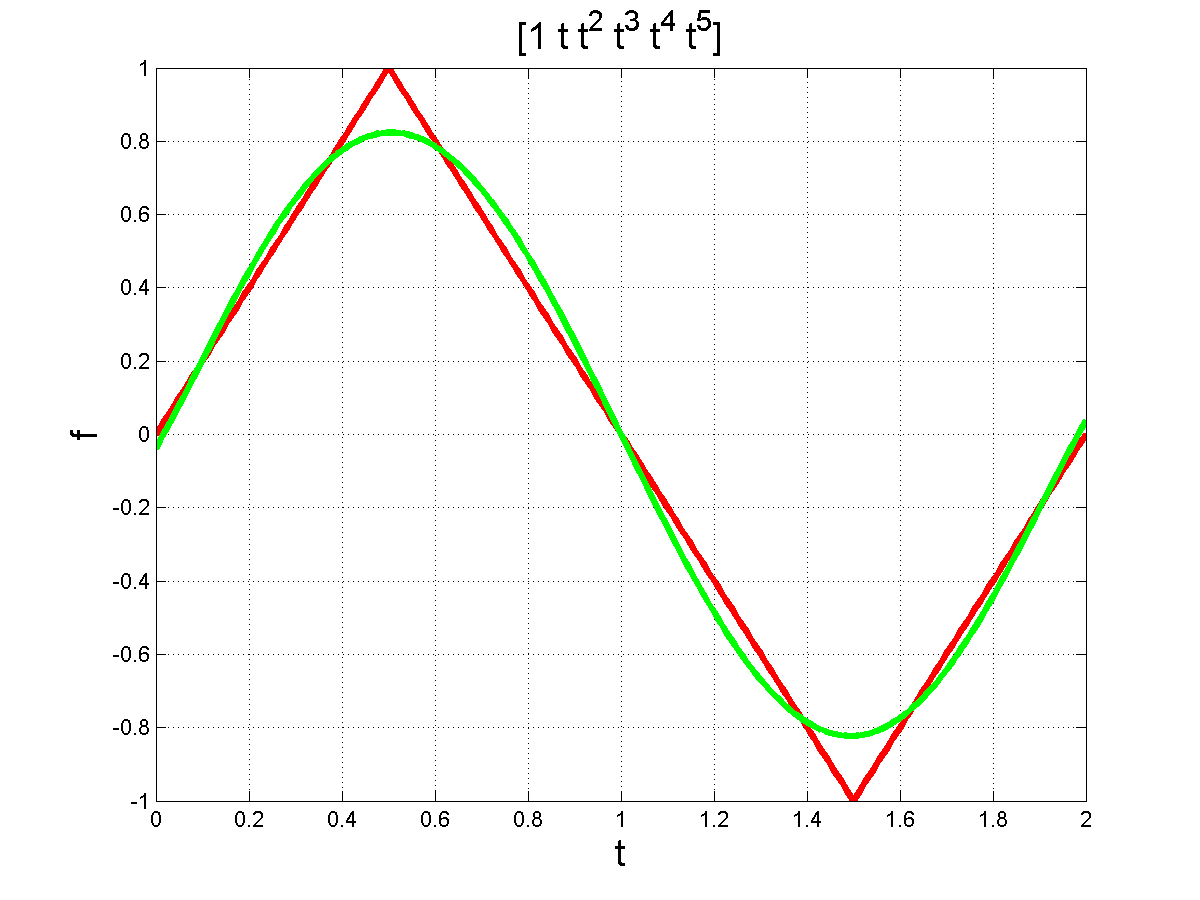
\includegraphics[width=0.6\textwidth]{../Prob8RegressionAgainstPolynomials.png}
\end{figure}

\item We write $\hat{f}(t_i)=\alpha_1 \sin(\pi t_i)+ \cdots + \alpha_5 \sin(5\pi t_i)$ and form the matrices
$$A=\left[\begin{array}{ccc} \sin(\pi t_1) & \cdots & \sin(5\pi t_1) \\
\vdots & & \vdots \\
\sin(\pi t_N) & \cdots & \sin(5\pi t_N)
\end{array}\right], b=\begin{bmatrix}f(t_1) \\ \vdots \\ f(t_N) \end{bmatrix} \text{and } \alpha=\begin{bmatrix}\alpha_1 \\ \vdots \\ \alpha_5 \end{bmatrix}$$
From the handout, we obtain
$$\hat{\alpha} = (A^T A)^{-1} A^T b =\begin{bmatrix}
0.8106 \\ 0.00 \\ -0.0901 \\ 0.00 \\ 0.0325 \end{bmatrix}$$

\begin{figure}[h]
\centering
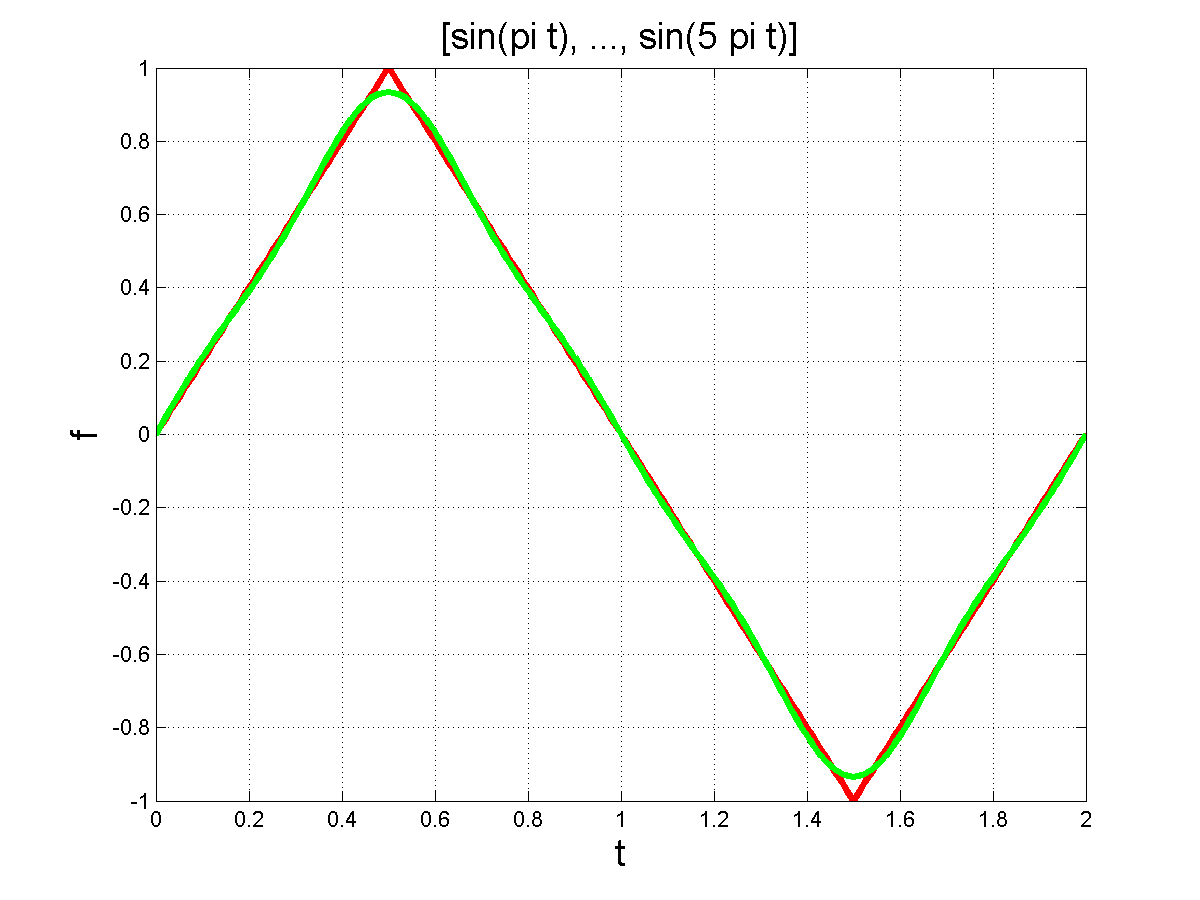
\includegraphics[width=0.6\textwidth]{../Prob8RegressionAgainstSinusoids.png}
\end{figure}

Here is the MATLAB code
\input{../Prob8.txt}
\end{enumerate}

\bigskip

\noindent \textbf{Problem 9:}
There is no "correct" choice for a basis. I chose $\{1,t,t^2,t^3\}$. \\
Repeating the results of Prob 8, I obtained
$$\hat{\alpha} = \begin{bmatrix}
0.0495 \\ -0.0847 \\ -1.8287 \\ 2.890 \end{bmatrix}$$
That is
$$\hat{f}(t)=0.0495-0.0847t-1.8287t^2+2.890t^3$$
I obtained
$$\frac{d\hat{f}_t}{dt}\Big|_{t=0.3} \approx -0.4$$

\begin{figure}[h]
\centering
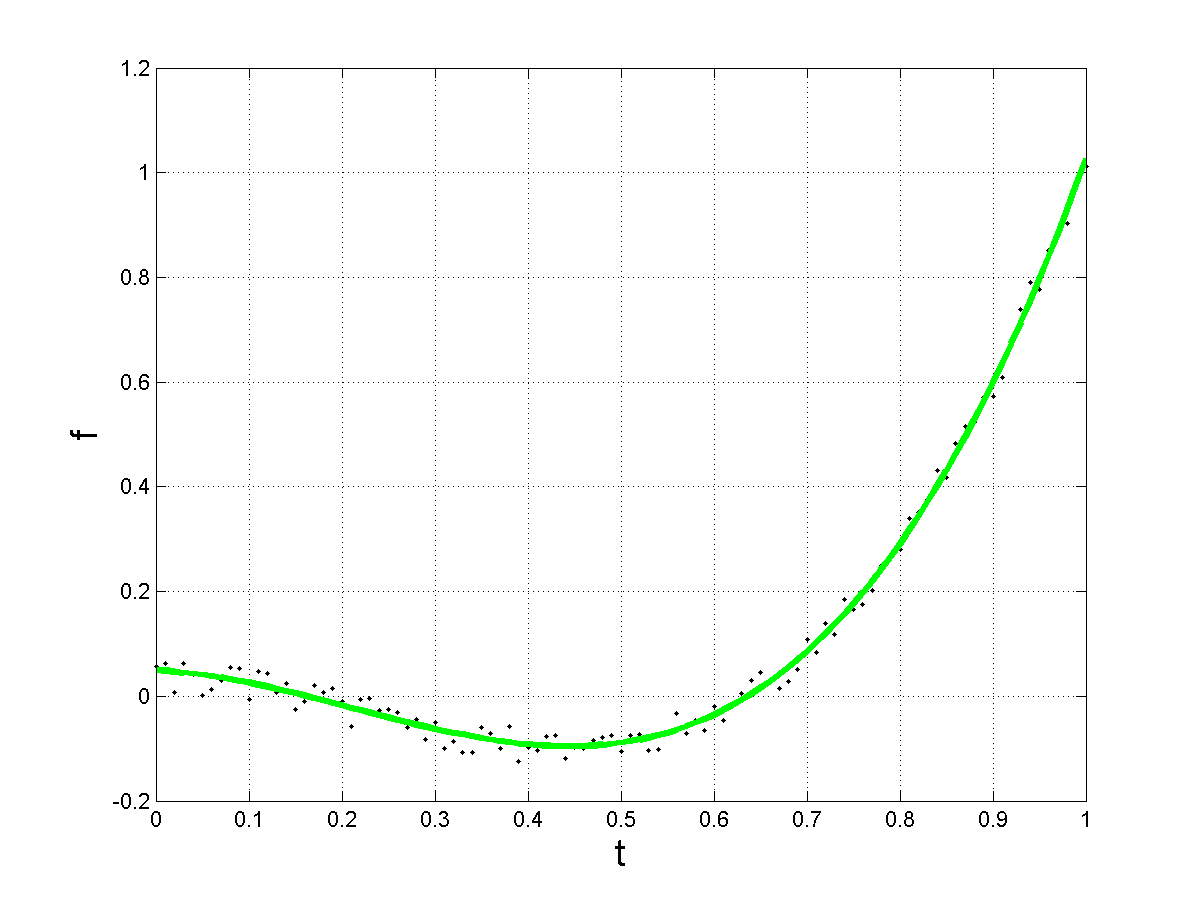
\includegraphics[width=0.58\textwidth]{../Prob9RegressionResult.png}
\end{figure}
Here is the MATLAB code
\input{../Prob9.txt}
\end{document} 